\section{User Guide}
This section contains information directed specifically to users. It contains clear descriptions of what inputs are needed and what effect they have. It should also help the user be able to use the model for the first time. Some possible examples are included below:

\subsection{Variable Definition and Code Description}
The variables in Table \ref{tabular:vars} are available for user input. Variables used by the module but not available to the user are not mentioned here. Variables with default settings do not necessarily need to be changed by the user, but may be.
\begin{table}[H]
	\caption{Definition and Explanation of Variables Used.}
	\label{tab:errortol}
	\centering \fontsize{10}{10}\selectfont
	\begin{tabular}{ | m{3cm}| m{3cm} | m{3cm} | m{6cm} |} % Column formatting, 
		\hline
		\textbf{Variable}   							& \textbf{LaTeX Equivalent} 	&		\textbf{Variable Type} & \textbf{Notes}			  \\ \hline
		spherHarm.maxDeg					&$l_{\text{max}}$		 	  & double & Default setting: 0"inertial\_state number of degree to use when calculating gravity effects using sperical harmonics.\\ \hline
		radEquator			   & $R_{\mathrm{ref}}^{l}$			& double & [m] Default setting: 0.0. 	This is the reference radius of the gravity body.\\ \hline
		muBody					& $\mu$ 		& double & [m3/s2] Default setting: 0.0f. This is the gravitational parameter of the body. Required Input to get any non-zero values out of the code.\\ \hline
		isCentralBody & N/A & bool & Default setting: False. Determines whether the body in question is the central (inertial) body.\\ \hline
		isDisplayBody & N/A & bool & Default setting: False. Determines whether the body in question is the focus of the visualization\\ \hline
		ephemTime & N/A & double & [s] Default setting: 0. The ephemeris time for the body in question \\ \hline
		ephIntTime & N/A & double & [s] Default setting: 0. Required Input. The integration time asociated with the ephem data. \\ \hline
		bodyInMsgName & N/A & string & Required Input. The name of the message with body data in the body frame. \\ \hline
		outputMsgName & N/A & string & Required Input. The name of the message containing ephemeris information in display frame \\ \hline
		planetEphemName & N/A & string & Required Input. An ephemeris name for the planet (user-named). \\ \hline
	\end{tabular}
	\label{tabular:vars}
\end{table}

\subsubsection{Code Diagram}

\begin{figure}[H]
	\centering 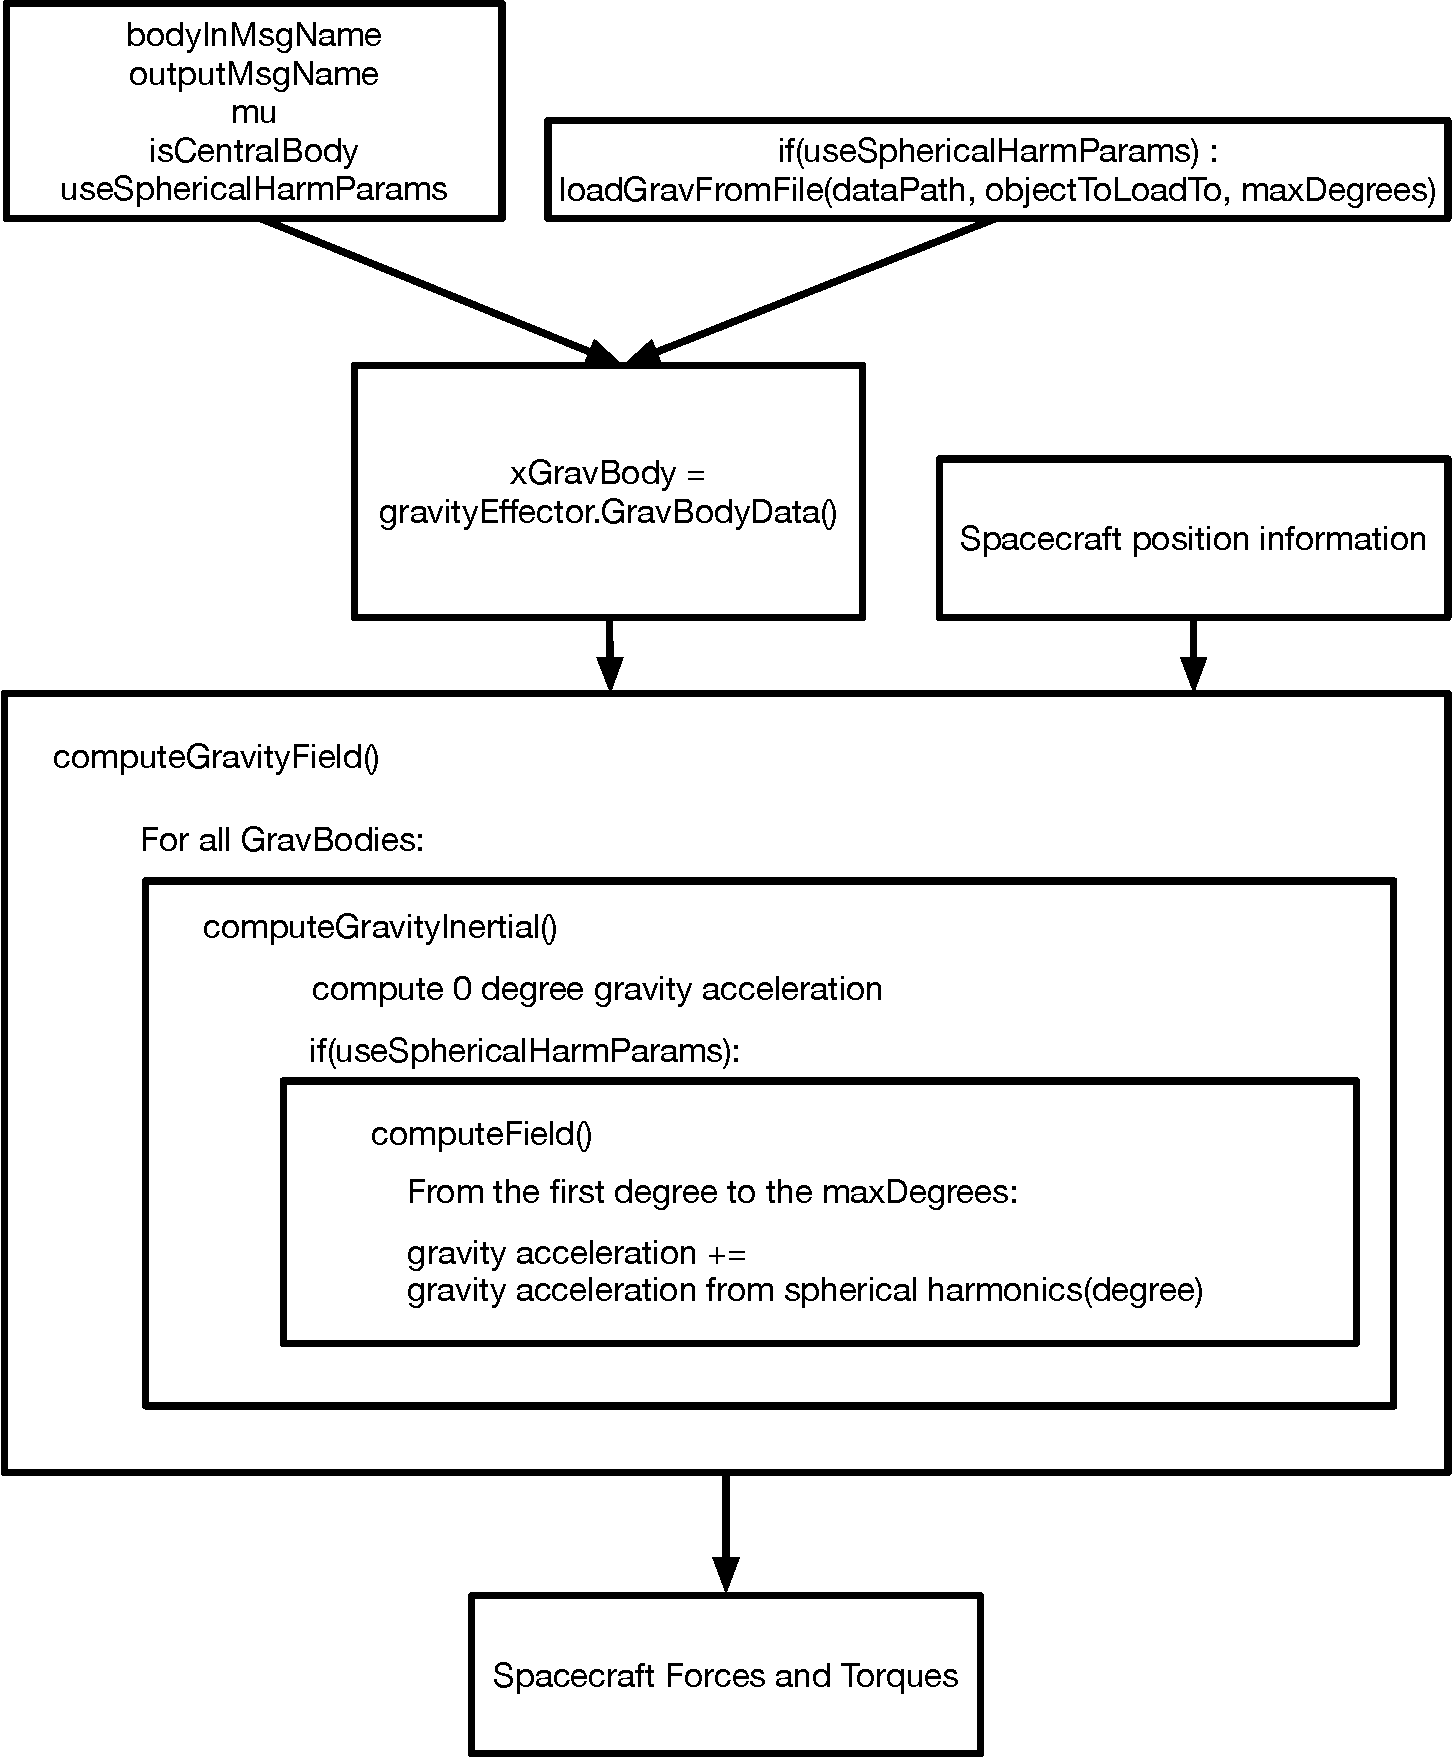
\includegraphics[height=0.8\textwidth, keepaspectratio]{Figures/codeFlow.pdf}
	\caption{A pseudo-code diagram demonstrating the flow of inputs and outputs in the gravity effector module.}
	\label{img:codeFlow}
\end{figure}

The diagram in Fig. \ref{img:codeFlow} demonstrates the basic iterative logic of the gravity effector module. There is extensive additional code that deals with things from the messaging system to transforming the spacecraft position from one frame to another. In general, the inputs shown must be given for each gravity body to be considered. There are, however, convenience functions which add the standard values of these inputs for common celestial bodies. An example is simIncludeGravbody.createEarth() in the test\_scenarioOrbitManeuver.py tutorial.

After the inputs are given for each gravity body, the computeGravityInertial() calculates the $0^{\textbf{th}}$ degree gravity term for each body and its effects on the spacecraft. If useSphericalHarmParams is True for a given body, then computeField() is called to calculate higher degree spherical harmonics terms for that body.
